In this final chapter we present the signal reconstruction efficiencies for the considered
 Hidden Valley
model depending on the masses and lifetimes of the exotic \Higgs and \X particles. 
We then unblind the data in the signal region and confront it with a background and hypothetical
 signal hypothesis. The data is consistent with the background only hypothesis, therefore we
compute upper limits depending on the reconstruction efficiency of the signal models.

\section{Long-lived particles reconstruction efficiency}
\label{sec:signalefficiency}

The signal events contain two \X bosons each decaying to $\qq$, therefore we define the \X bosons 
 efficiency times acceptance ($\epsilon A$) as:
\begin{equation}
\epsilon A= \frac{N_{X reconstructed}}{2N_{events}}
\end{equation}

where the \X bosons acceptance $A$ has been defined in Section \ref{sec:sigsensitivity}. 
Table \ref{tab:sigeff} presents the acceptance and efficiency for
reconstructing \X boson candidates as a function of the \Higgs and \X particles masses for different 
mean lifetimes of the \X particles.

\begin{table}[htbp]
\caption{
Signal acceptance and reconstruction efficiency ($\epsilon$) for $\X \to \qq$ in simulated signal models.
The trigger and reconstruction efficiencies are both included in the efficiency.
The uncertainties are statistical only.\label{tab:sigeff}}
\centering
\begin{tabular}{llcccc}
\hline
$\Higgs$ [GeV] & $\X$ [GeV] & c$\tau$ [cm] & $\langle L_{xy} \rangle$ [cm] & Acceptance [\%] & $\epsilon$ [\%] \\
\hline
200 & 50 & 2 & 3 & $9.1\pm0.2$ & $1.5\pm0.3$ \\
200 & 50 & 20 & 30 & $7.3\pm0.2$ & $0.8\pm0.2$ \\
\hline
400 & 50 & 0.8 & 2.6 & $35.2\pm0.4$ & $8.8\pm0.4$ \\
400 & 50 & 8 & 26 & $31.3\pm0.4$ & $4.4\pm0.3$ \\
400 & 50 & 80 & 260 & $7.2\pm0.2$ & $1.6\pm0.4$ \\
\hline
400 & 150 & 4 & 3 & $59.9\pm0.4$ & $15.9\pm0.4$ \\
400 & 150 & 40 & 30 & $51.5\pm0.4$ & $6.7\pm0.3$ \\
400 & 150 & 400 & 300 & $13.6\pm0.3$ & $1.7\pm0.3$ \\
\hline 
1000 & 150 & 1 & 2.5 & $74.6\pm0.4$ & $37.7\pm0.4$ \\
1000 & 150 & 10 & 25 & $66.8\pm0.4$ & $25.3\pm0.4$ \\ 
1000 & 150 & 100 & 250 & $15.7\pm0.3$ & $14.4\pm0.7$ \\
\hline 
1000 & 350 & 3.5 & 2.9 & $89.0\pm0.2$ & $39.0\pm0.4$ \\
1000 & 350 & 35 & 29 & $76.9\pm0.3$ & $22.0\pm0.4$ \\
1000 & 350 & 350 & 290 & $19.4\pm0.3$ & $11.0\pm0.5$ \\
\hline
\end{tabular}
\end{table}

\X particle reconstruction efficiencies presented in Table \ref{tab:sigeff} 
are applicable to a model where \X particles decay with equal branching fractions to 
u, d, s, c and b quark flavor pairs.
Table \ref{tab:sigeffflavor} shows the \X particle reconstruction efficiencies separately for 
\X decaying light quarks (u,d,s) and
heavier quarks c and b. 

\begin{table}[htbp]
\caption{
Signal reconstruction efficiency (trigger and offline) for $\X \to \qq$ in simulated signal models for light (uds) and heavy (c and b) quark flavours.  The uncertainties are statistical only. \label{tab:sigeffflavor}}
\centering
\begin{tabular}{llccccc}
\hline
$\Higgs$ [GeV] & $\X$ [GeV] & c$\tau$ [cm] & $\langle L_{xy} \rangle$ [cm] & $\epsilon_{uds}$ [\%] & $\epsilon_{c} [\%] $ & $\epsilon_{b}$ [\%]\\
\hline
200 & 50 & 2 & 3 & $1.9\pm0.4$ & $1.3\pm0.6$ & $0.5\pm0.4$ \\
200 & 50 & 20 & 30 & $0.9\pm0.3$ & $0.7\pm0.5$ & $0.5\pm0.4$ \\
\hline
400 & 50 & 0.8 & 2.6 & $10.5\pm0.5$ & $8.6\pm0.8$ & $4.2\pm0.6$ \\
400 & 50 & 8 & 26 & $5.3\pm0.4$ & $4.0\pm0.6$ & $2.5\pm0.5$ \\
400 & 50 & 80 & 260 & $1.9\pm0.5$ & $1.3\pm0.7$ & $0.9\pm0.6$ \\
\hline
400 & 150 & 4 & 3 &  $18.2\pm0.5$ & $15.7\pm0.8$ & $11.2\pm0.7$ \\
400 & 150 & 40 & 30 & $7.5\pm0.4$ & $6.5\pm0.6$ & $5.4\pm0.5$ \\
400 & 150 & 400 & 300 & $2.1\pm0.4$ & $1.5\pm0.6$ & $1.2\pm0.5$ \\
\hline
1000 & 150 & 1 & 2.5 & $39.3\pm0.5$ & $38.6\pm0.9$ & $34.5\pm0.9$ \\
1000 & 150 & 10 & 25 & $25.6\pm0.5$ & $26.2\pm0.9$ & $25.2\pm0.9$ \\
1000 & 150 & 100 & 250 & $15.0\pm0.9$ & $15.7\pm2.0$ & $13.0\pm1.0$ \\
\hline
1000 & 350 & 3.5 & 2.9 &  $40.6\pm0.5$ & $40.4\pm0.9$ & $36.3\pm0.8$ \\
1000 & 350 & 35 & 29 & $22.8\pm0.5$ & $22.1\pm0.8$ & $21.1\pm0.8$ \\
1000 & 350 & 350 & 290 & $11.9\pm0.7$ & $11.0\pm1.0$ & $9.4\pm1.0$ \\
\hline
\end{tabular}
\end{table}

\begin{figure}[htbp]
\centering
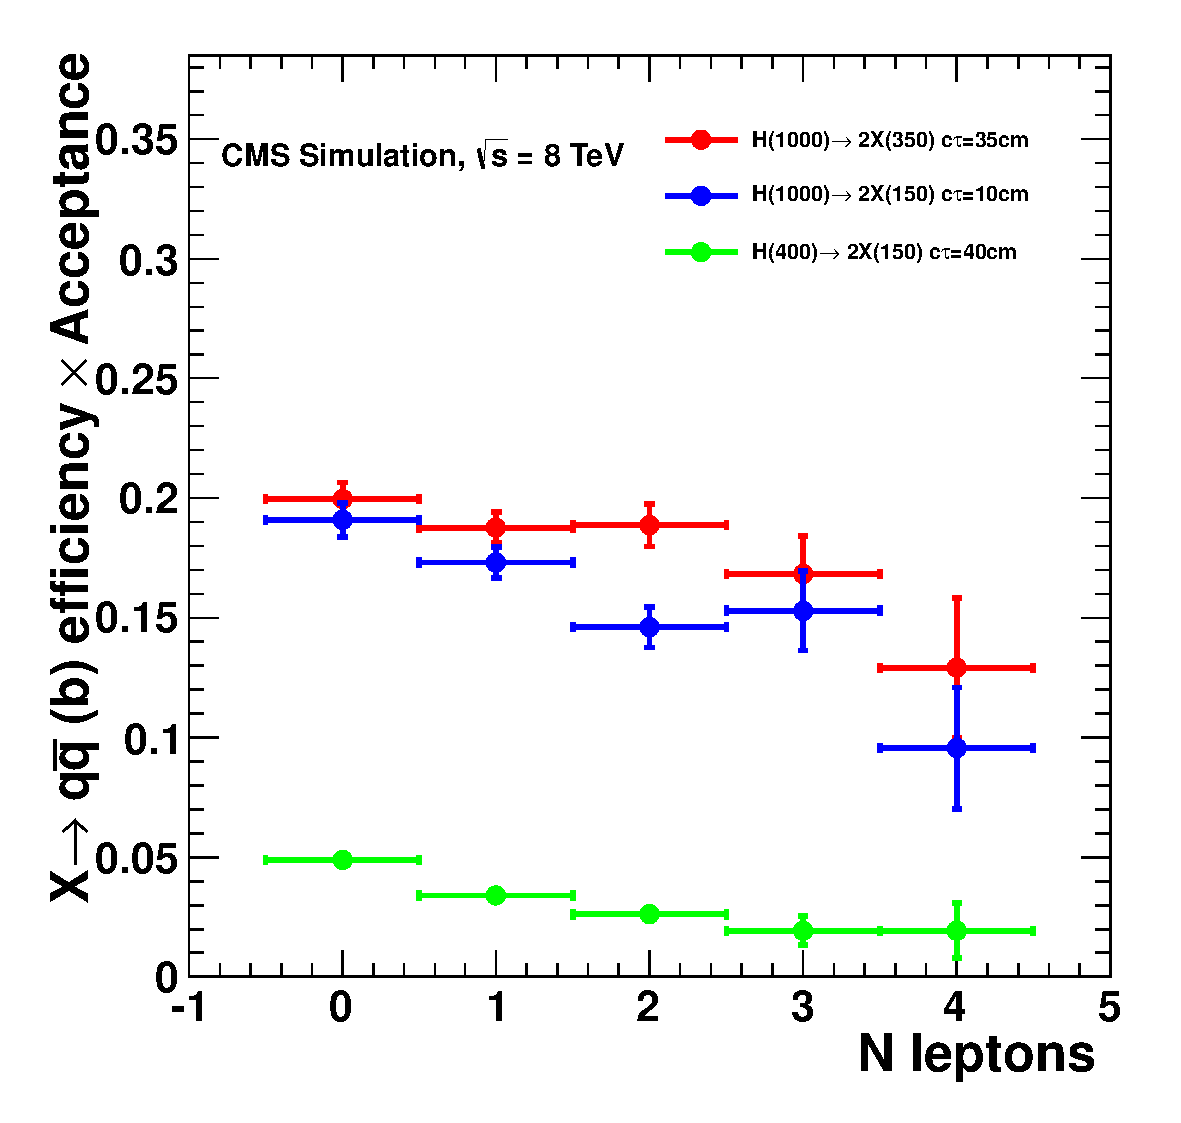
\includegraphics[width=0.49\textwidth]{plots/signal/effNLepb.pdf}
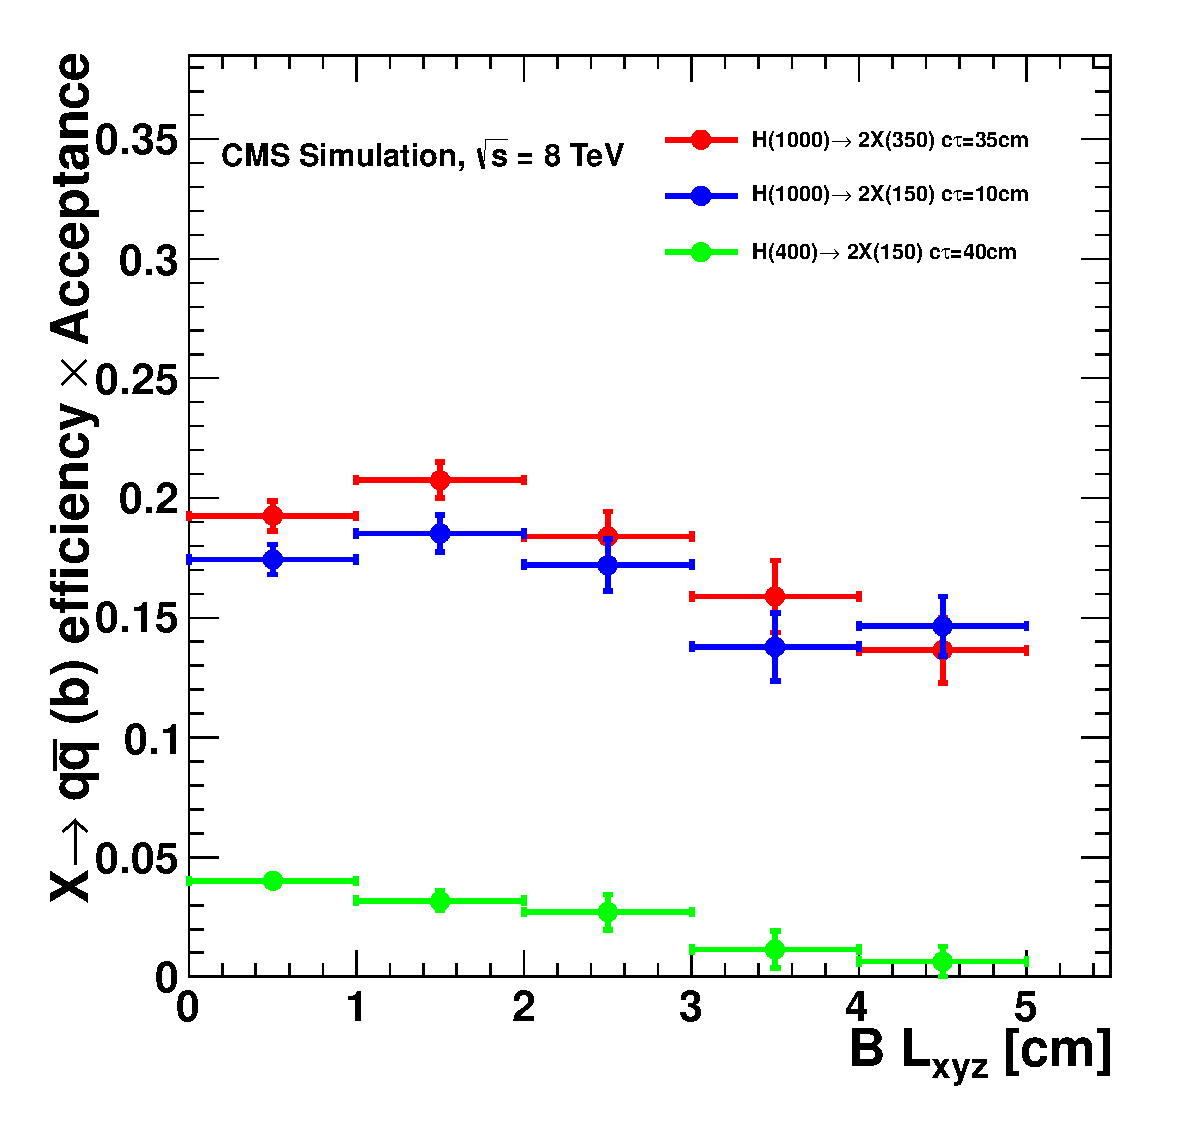
\includegraphics[width=0.49\textwidth]{plots/signal/effBlxyzb.pdf}
\caption{$\X \to \bbbar$ reconstruction efficiency as a function of the total number of leptons 
originating from B mesons/baryons (left) and as a function of B mesons/baryons decay length. Only selected 
mass points are shown. The samples correspond to the mixture of the three generated mean 
lifetimes of the \X bosons. \label{fig:effb}}
\end{figure}

The c and b quarks hadronize mostly into D or B mesons respectively.
 Unlike the light quark mesons a significant fraction of heavy flavor
mesons decays semi-leptonically reducing the track multiplicity of the jets and also reducing the jet momenta
 due to the missing energy of associated neutrinos. 
Additionally the D or B mesons split the dijet vertex due to their intrinsic lifetime.
Figure \ref{fig:effb} shows the reconstruction efficiency of the $\X \to \bbbar$ candidates as a function
of the total number of leptons originating from the \bbbar pair and as a function of the B mesons decay
length. The reconstruction efficiency is affected by both, the presence of leptons among
the decay products, and the
B mesons decay length.

In order to visualize the capabilities of the CMS detector for reconstructing long-lived particles decaying to 
dijets, 
the reconstructed dijet mass and $L_{xy}$ distributions for selected signal models are shown in Figure
\ref{fig:signal}. We assume the cross-section of the $\Higgs \to 2\X$ process to be 1 pb and the branching 
ratio to quarks ($\X \to \qq$) to be 100\%.

\begin{figure}[htbp]
\centering
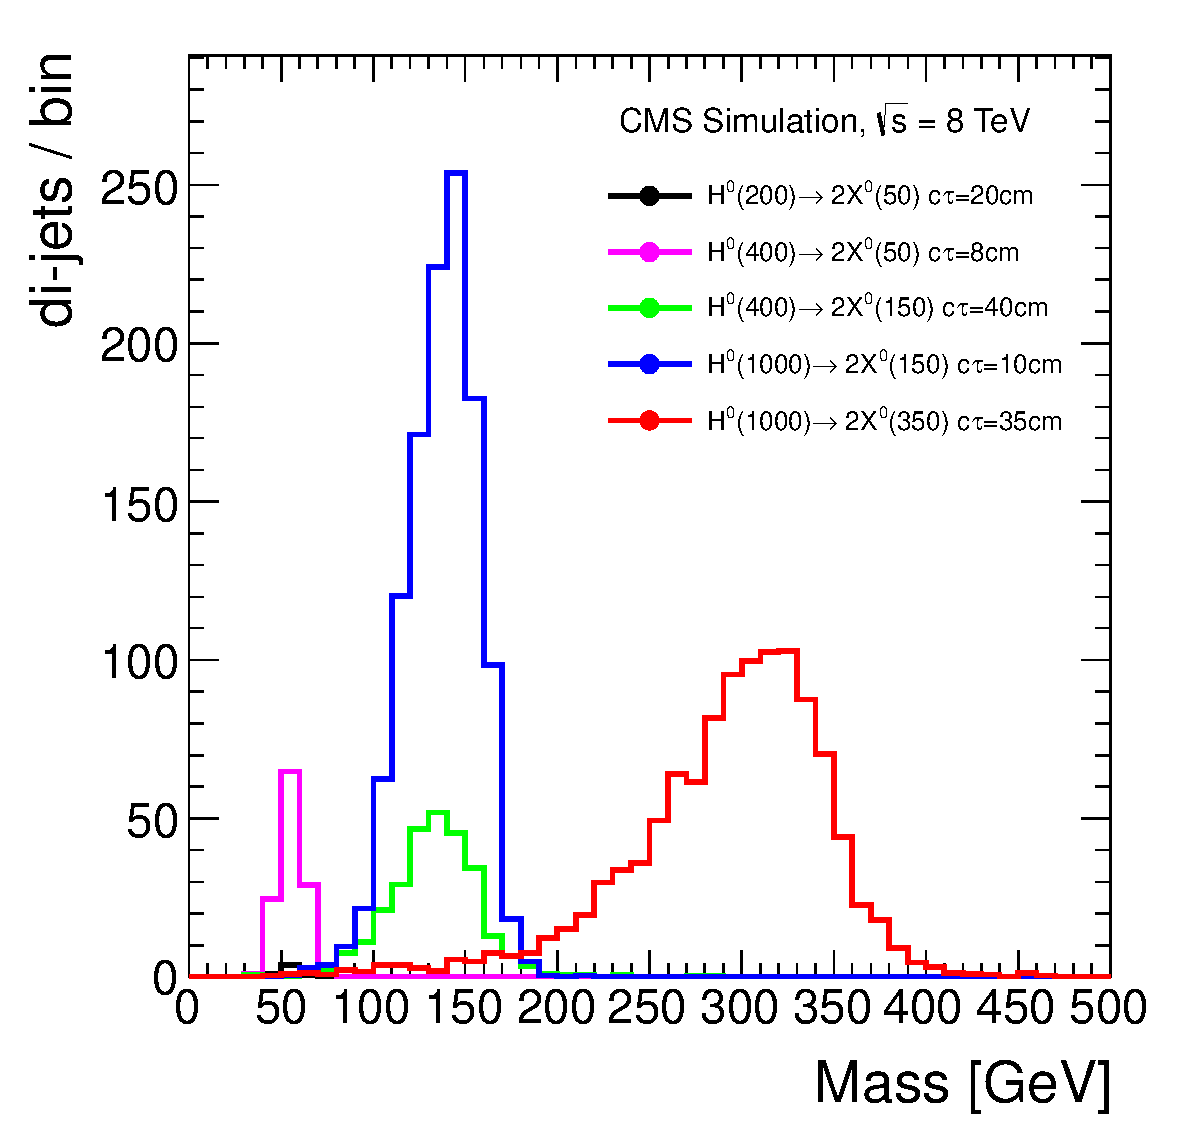
\includegraphics[width=0.49\textwidth]{plots/signal/mass.pdf}
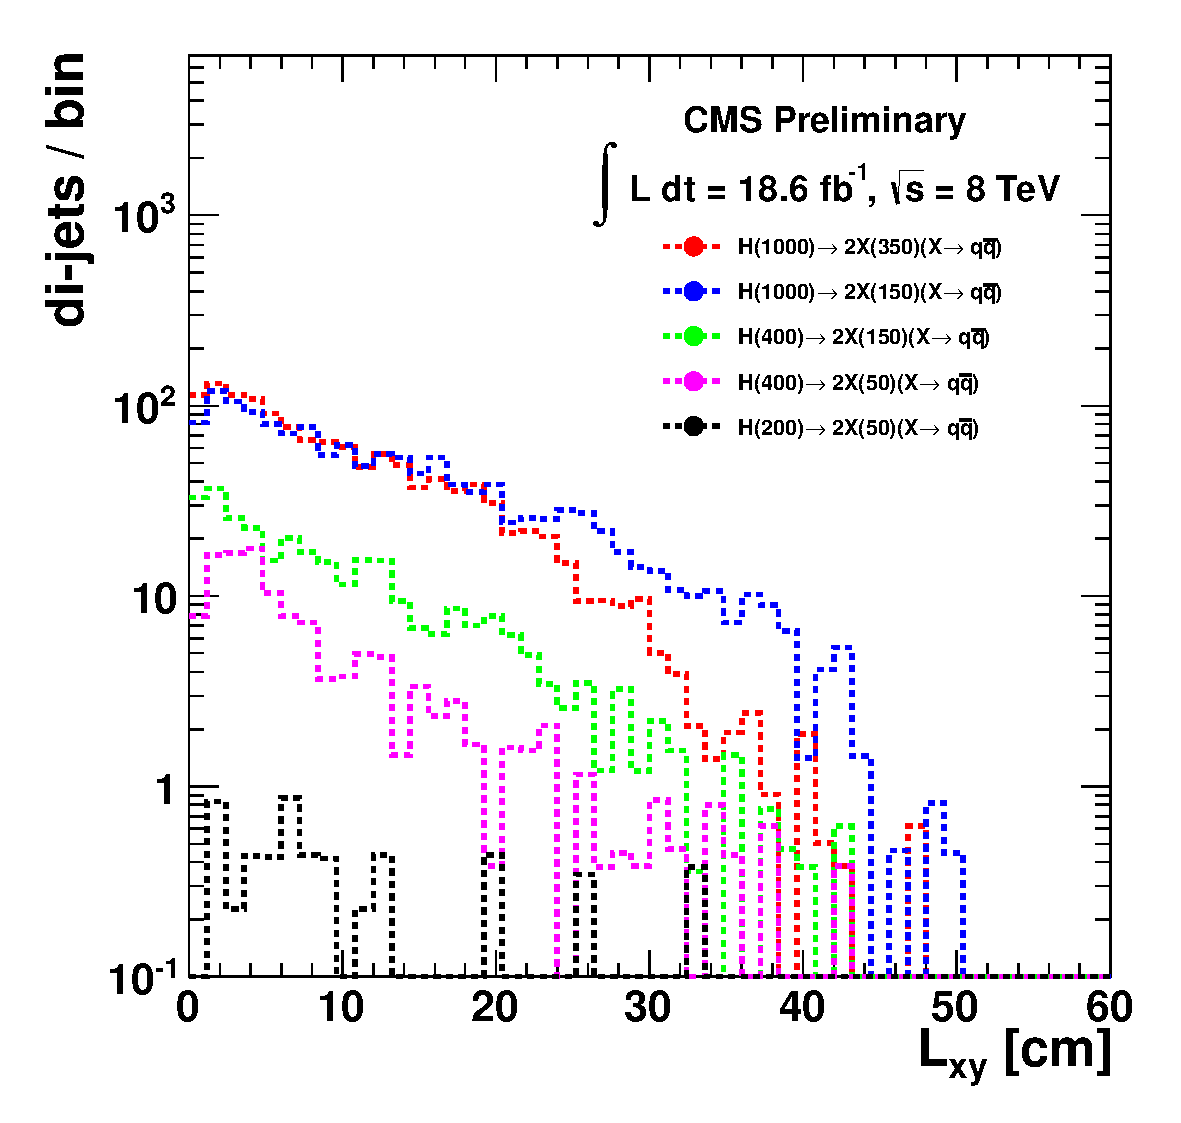
\includegraphics[width=0.49\textwidth]{plots/signal/Lxy.pdf}
\caption{The reconstructed dijet mass and $L_{xy}$ for selected signal models; central lifetime out of the three available is presented.\label{fig:signal}}
\end{figure}

\section{Data in the signal region}
\label{sec:fullunblinding}

Table \ref{tab:fullunblinding} summarizes the observed candidate counts in the signal region for the optimized 
selections detailed in Section \ref{sec:cutvalues}. Data is found in good agreement with the 
background only hypothesis. In addition, the two selected candidates are examined using event displays
and are found consistent with background candidates as described in Figure \ref{fig:eventDisplays}.  

\begin{table}[htbp]
\centering
\begin{tabular}{|l|c|c|}
\hline
$\bf L_{xy}$ \bf selection & \bf low & \bf high \\
\hline
\bf Predicted Background & $ 1.60\pm0.58(stat+sys)$ & $ 1.14\pm0.54(stat+sys)$ \\
\hline
\bf Observed candidates & 2 & 1 \\ 
\hline
\end{tabular}
\caption{Observed candidates and predicted background for the optimized selections.\label{tab:fullunblinding}}
\end{table}

\begin{figure}
\centering
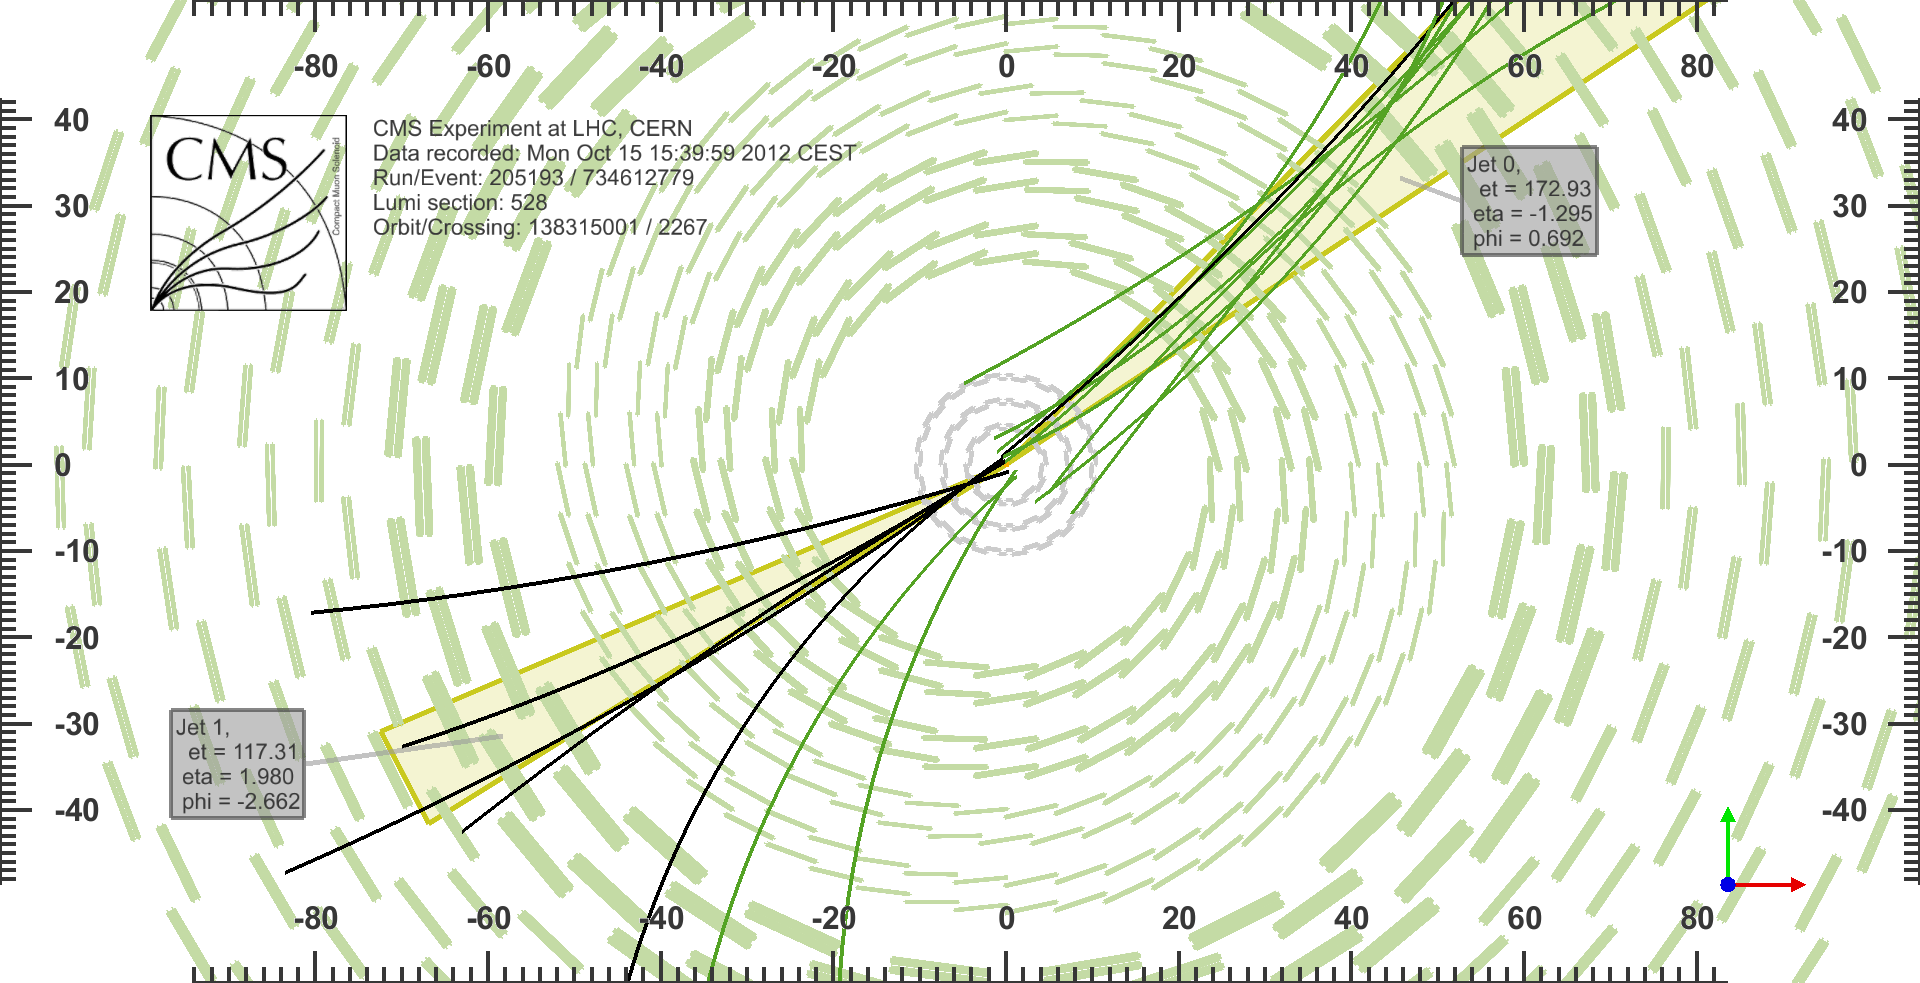
\includegraphics[width=0.9\textwidth]{plots/displays/candidate1_display.png}
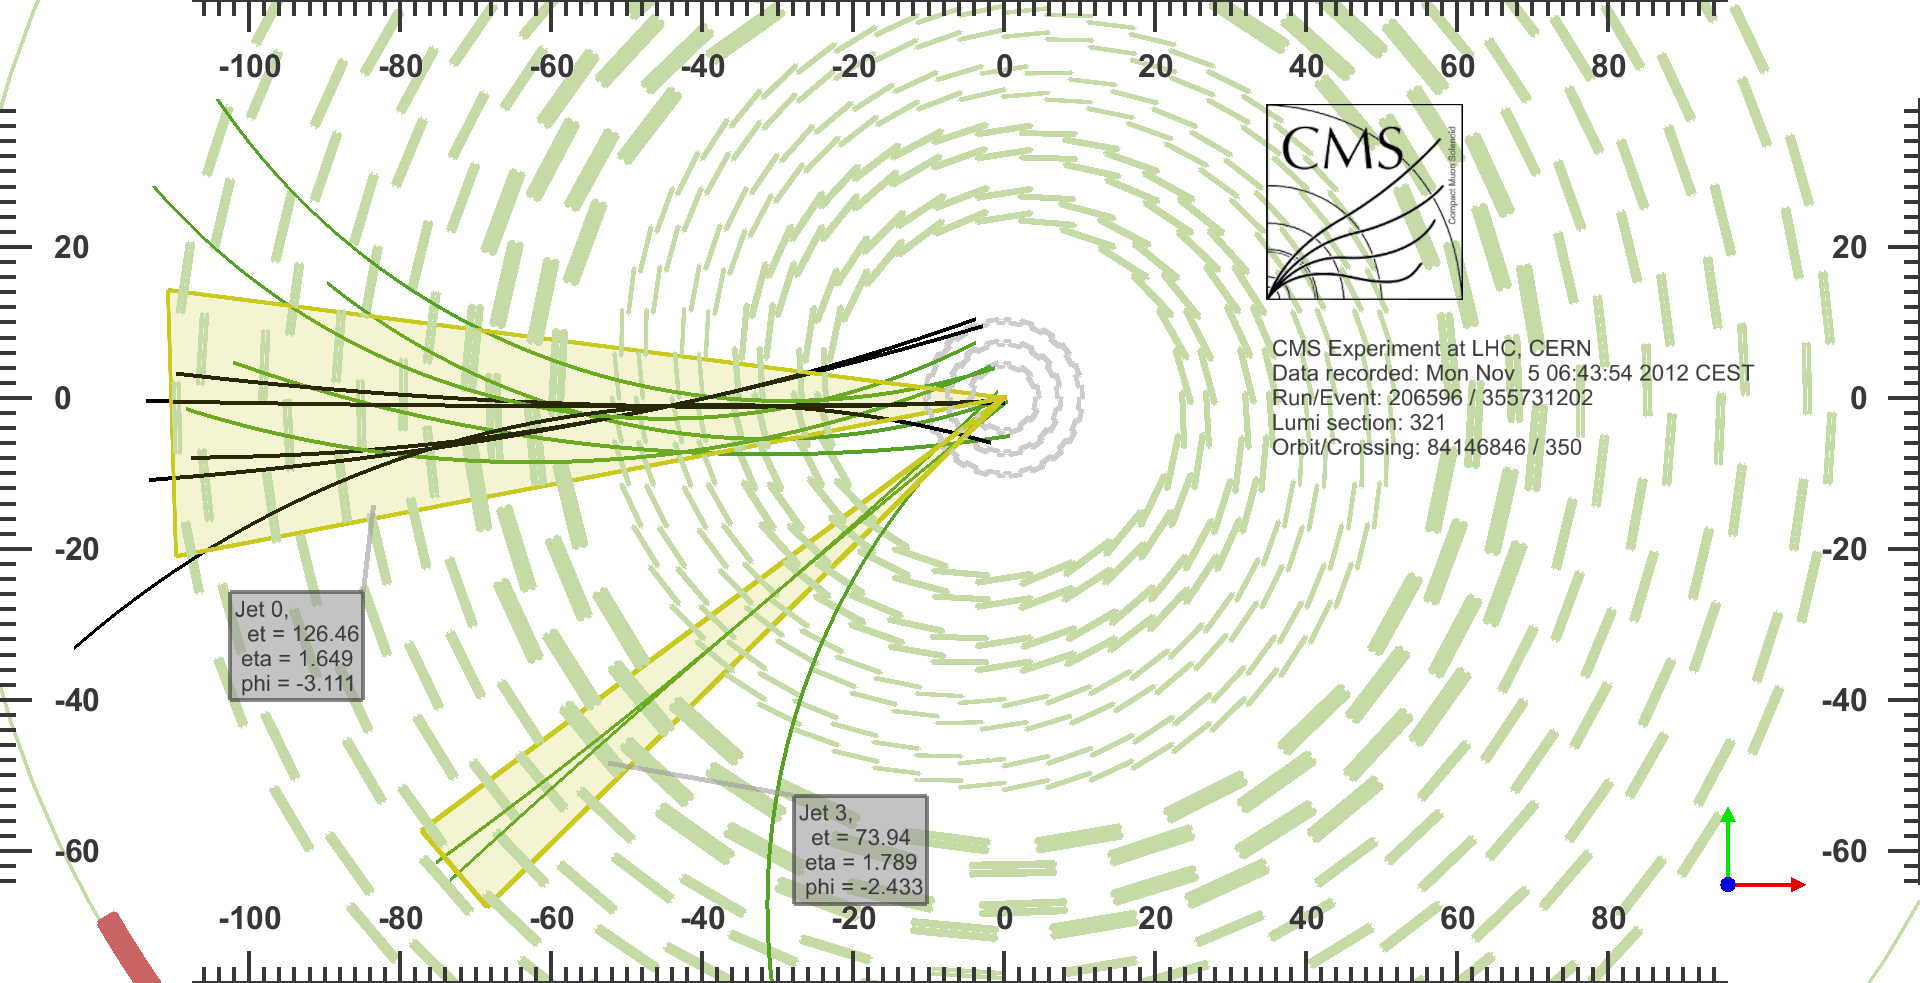
\includegraphics[width=0.9\textwidth]{plots/displays/candidate2_display.png}

\caption{Event displays of the two candidates passing the optimized selection where only the selected di-jet pair
 (yellow cones) and 
the associated tracks (curved lines) are shown, other objects being removed. The tracks that fit the secondary 
vertex are coloured black.  
Candidate 1 (top) with dijet invariant mass of 770 \GeV, which 
passes only the {\it low $L_{xy}$} selection, 
contains a secondary vertex, displaced transversely by 5 \cm, containing 5 tracks from one jet and 1 track
from the other. The 5 track vertex is consistent with a vertex of a B meson with invariant mass below 5 \GeV.
Candidate 2 (bottom) with dijet invariant mass of 75\GeV, 
which passes both {\it low} and {\it high $L_{xy}$} selections, contains a secondary vertex
, displaced transversely by 44 \cm, containing 5 tracks where 2 of these tracks are
associated to both jets due to the jets being nearby. The vertex invariant mass is low and its position
 coincides with one of the silicon 
tracker layers being consistent with a nuclear interaction vertex. \label{fig:eventDisplays}}
\end{figure} 



\section{Limits}
\label{sec:limits}

We set 95\% confidence level
(CL) upper limits for a counting experiment
using the CL$_\mathrm{s}$ method \cite{Read:2002hq, Junk:1999kv}. The limit calculation
takes into account the systematic uncertainties described in Chapter 
\ref{chap:systematics} by introducing
a nuisance parameter for each uncertainty, marginalised by a log-normal prior distribution.

As a first step, upper limits are placed on the mean number of \X bosons ($N_\X$) that could pass
the selection requirements. The resulting observed upper limits on $N_\X$ are 4.6 candidates
for the {\it low} $L_{xy}$ selection and 3.7 candidates for the {\it high} selection.
 These limits are independent
of the particular model assumed for \X boson production.


Secondly, an upper limit is quoted on the cross section
to produce $\Higgs \to 2\X$ times the branching fraction squared, $B^2$, for \X to decay into $\qq$.
The expected number of signal dijet candidates passing the selection can be expressed as:
\begin{equation}
N_\X \geq 2 \mathcal{L}\epsilon A\sigma B^2
\end{equation}
where $\mathcal{L}$ is the integrated luminosity, $A$ is the acceptance,
$\epsilon$ is the efficiency to reconstruct \X boson candidates
(Table \ref{tab:sigeff}), $\sigma$ is the production cross-section of the heavy resonance decaying to \X,
$B$ is the branching fraction of $\X$ to dijets, and the factor of 2 reflects the 2 $\X$ decays in each event.
 The non-equality arises from the fact that when the branching
fraction $B$
is smaller than 1, there is an additional contribution from events where only one \X boson decayed to dijets.
The limits will therefore be exact when $B=1$ and conservative when $B$ is smaller than 1.
The observed and
expected limits are shown in Figure \ref{fig:limits}. In order to expand the number of tested models,
the lifetime distributions of the signal MC candidates are reweighted to
different mean values, namely $0.4\tau$, $0.6\tau$, and $1.4\tau$ for every
lifetime value $\tau$ and mass combination listed
in Table \ref{tab:sigeff}.
Candidates are weighted using event based weights computed as the product
 of weights assigned to each $\X$ candidate in the event.
The reweighted signal reconstruction efficiencies are then used
to compute the expected and observed limits for these additional mean lifetime values.

\begin{figure}[htbp]
\centering
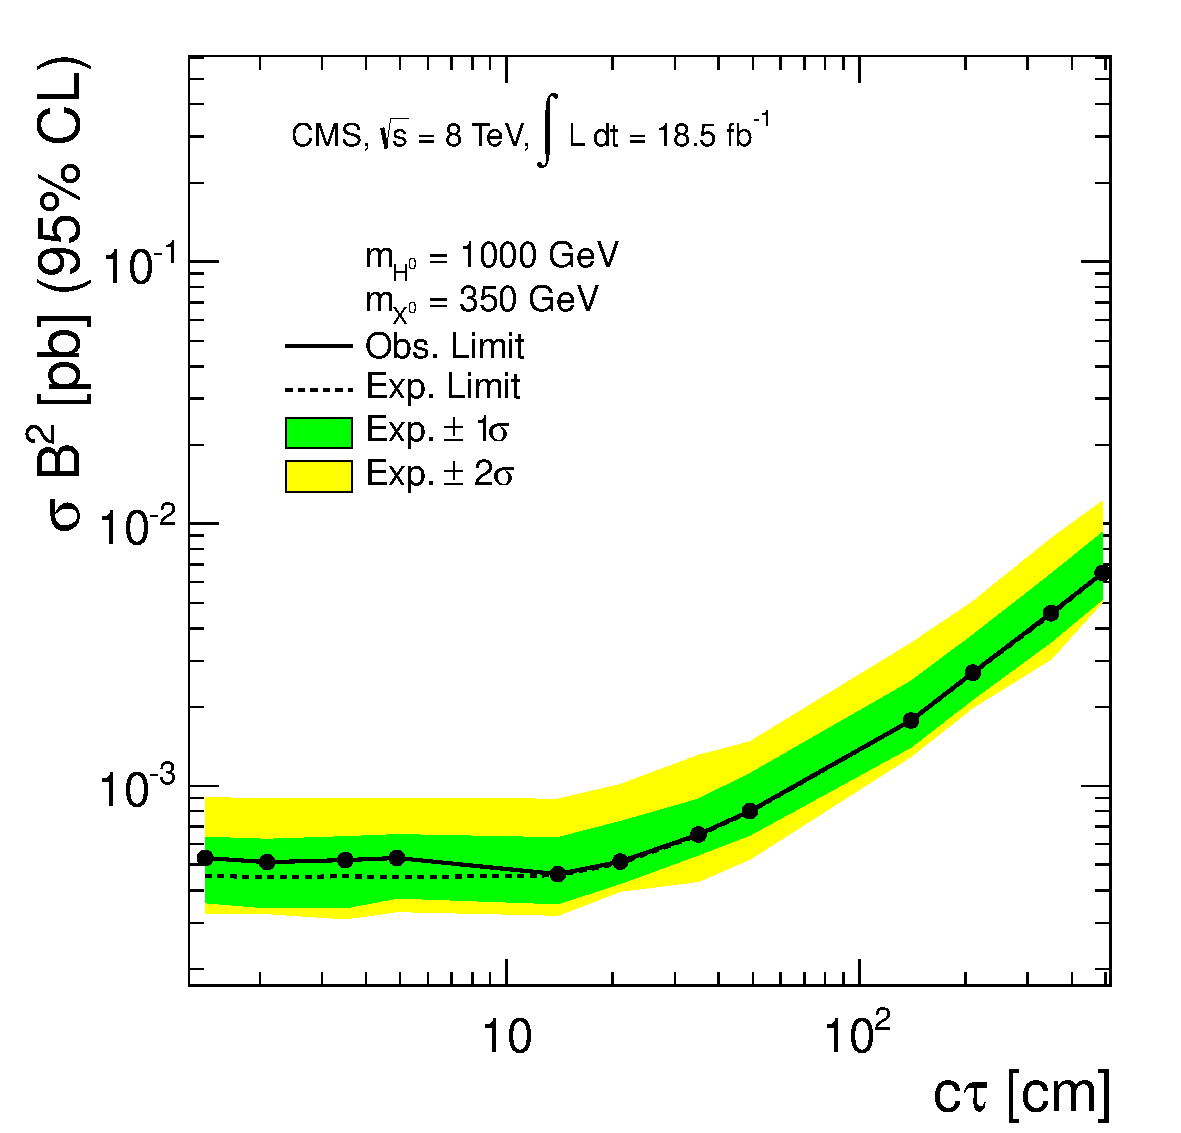
\includegraphics[width=0.49\textwidth]{plots/limits/1000_350e.pdf}
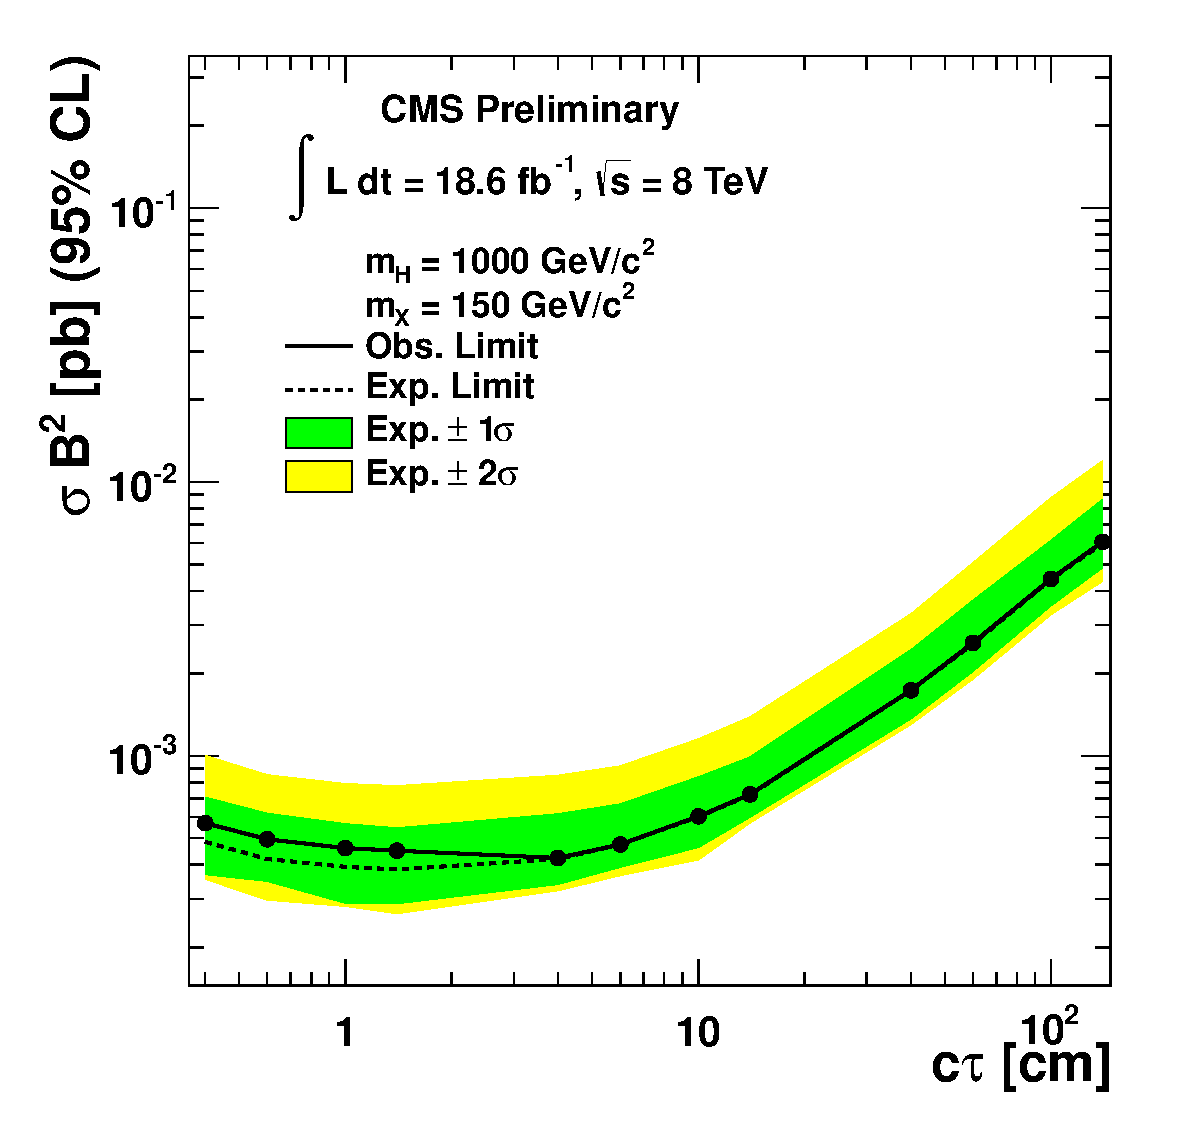
\includegraphics[width=0.49\textwidth]{plots/limits/1000_150e.pdf} 
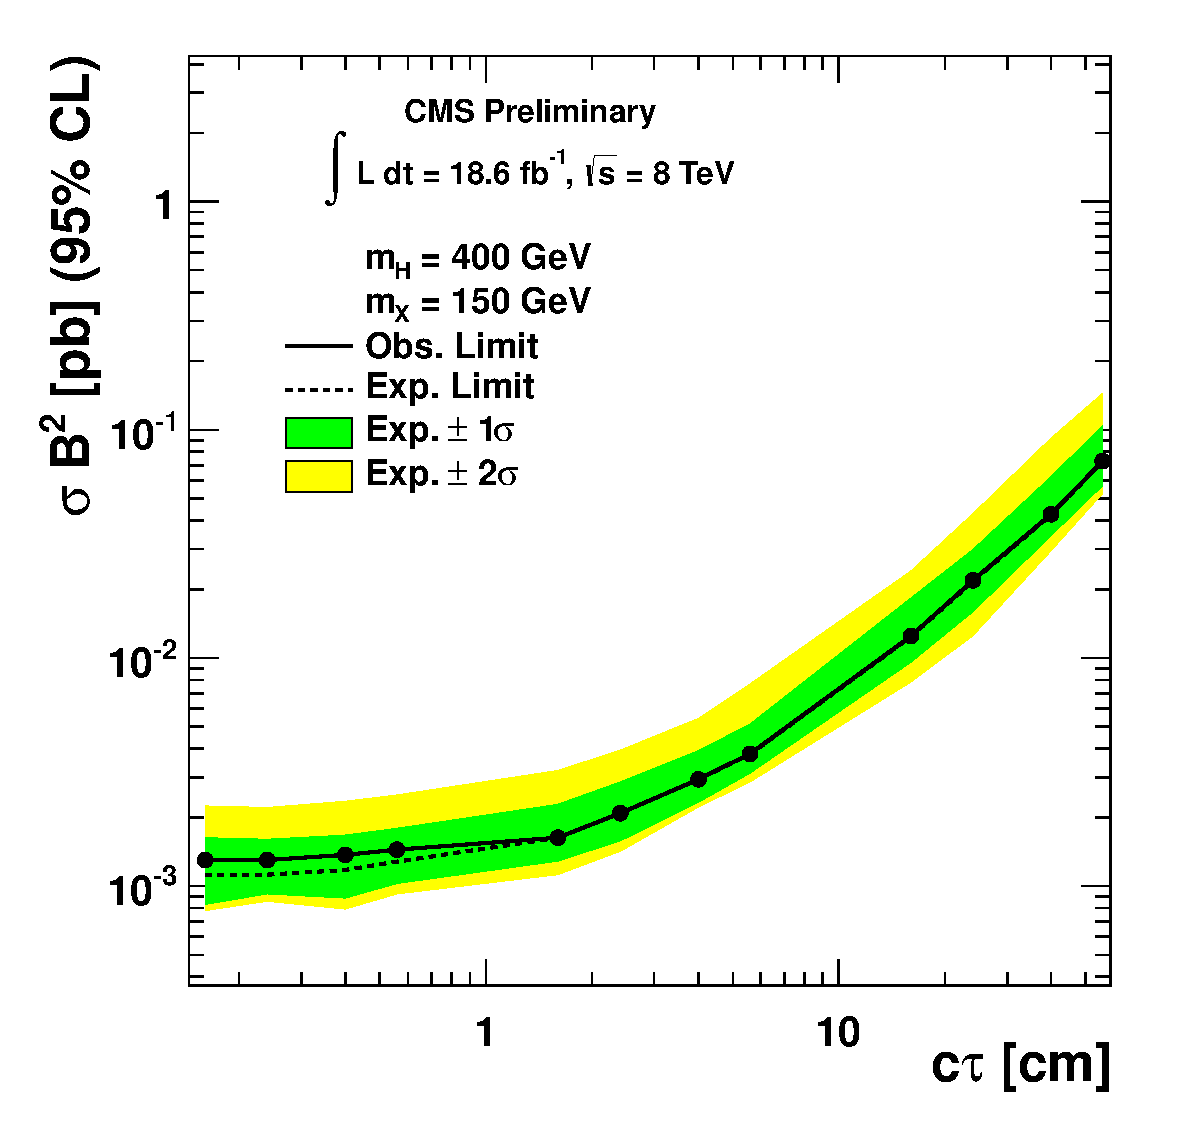
\includegraphics[width=0.49\textwidth]{plots/limits/400_150e.pdf}
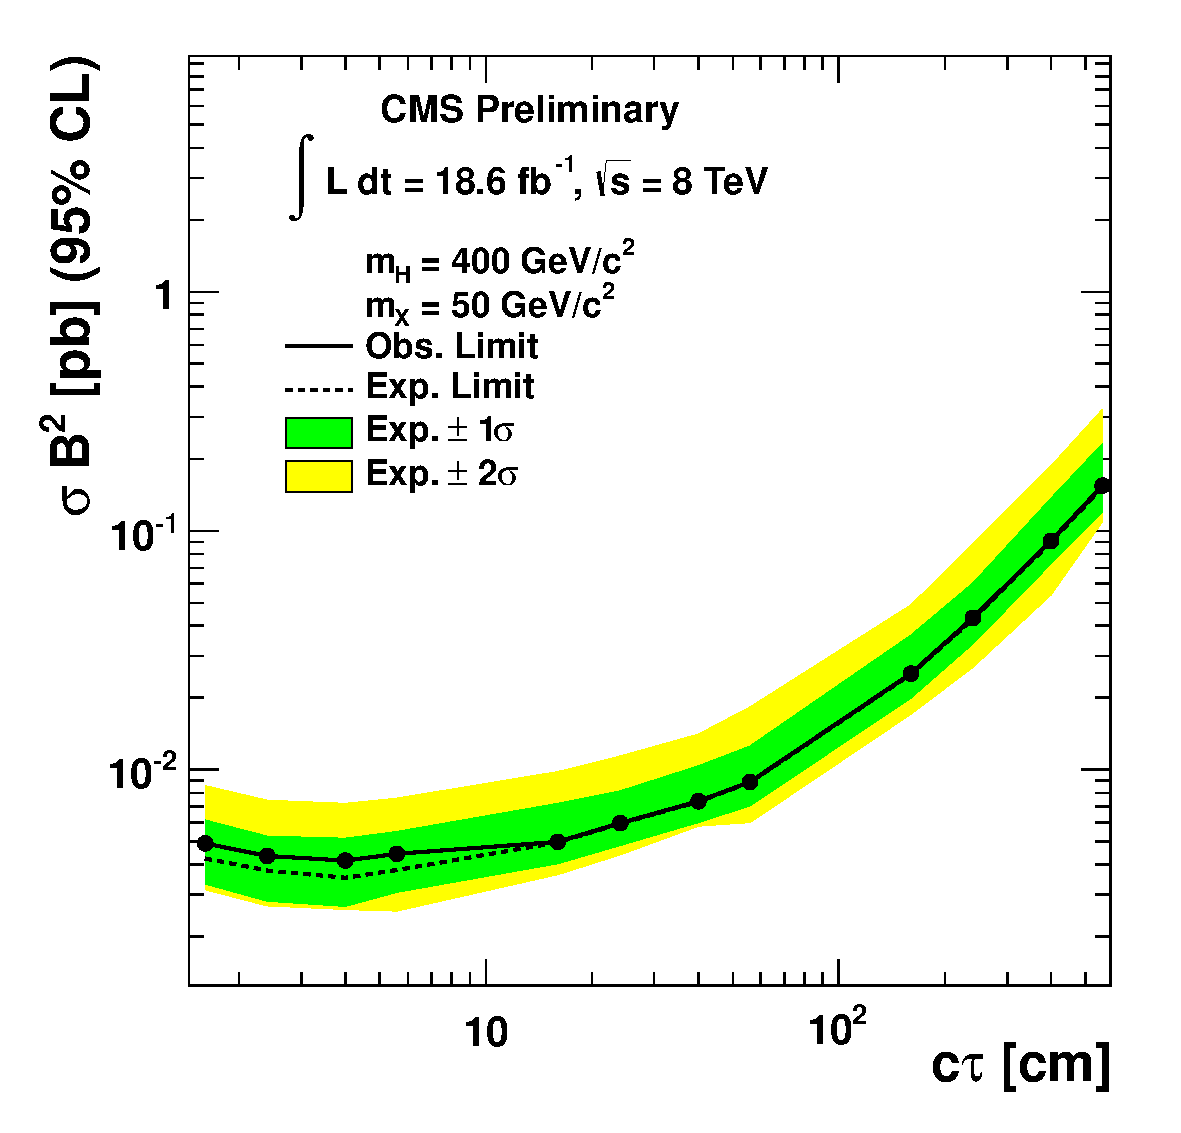
\includegraphics[width=0.49\textwidth]{plots/limits/400_50e.pdf} 
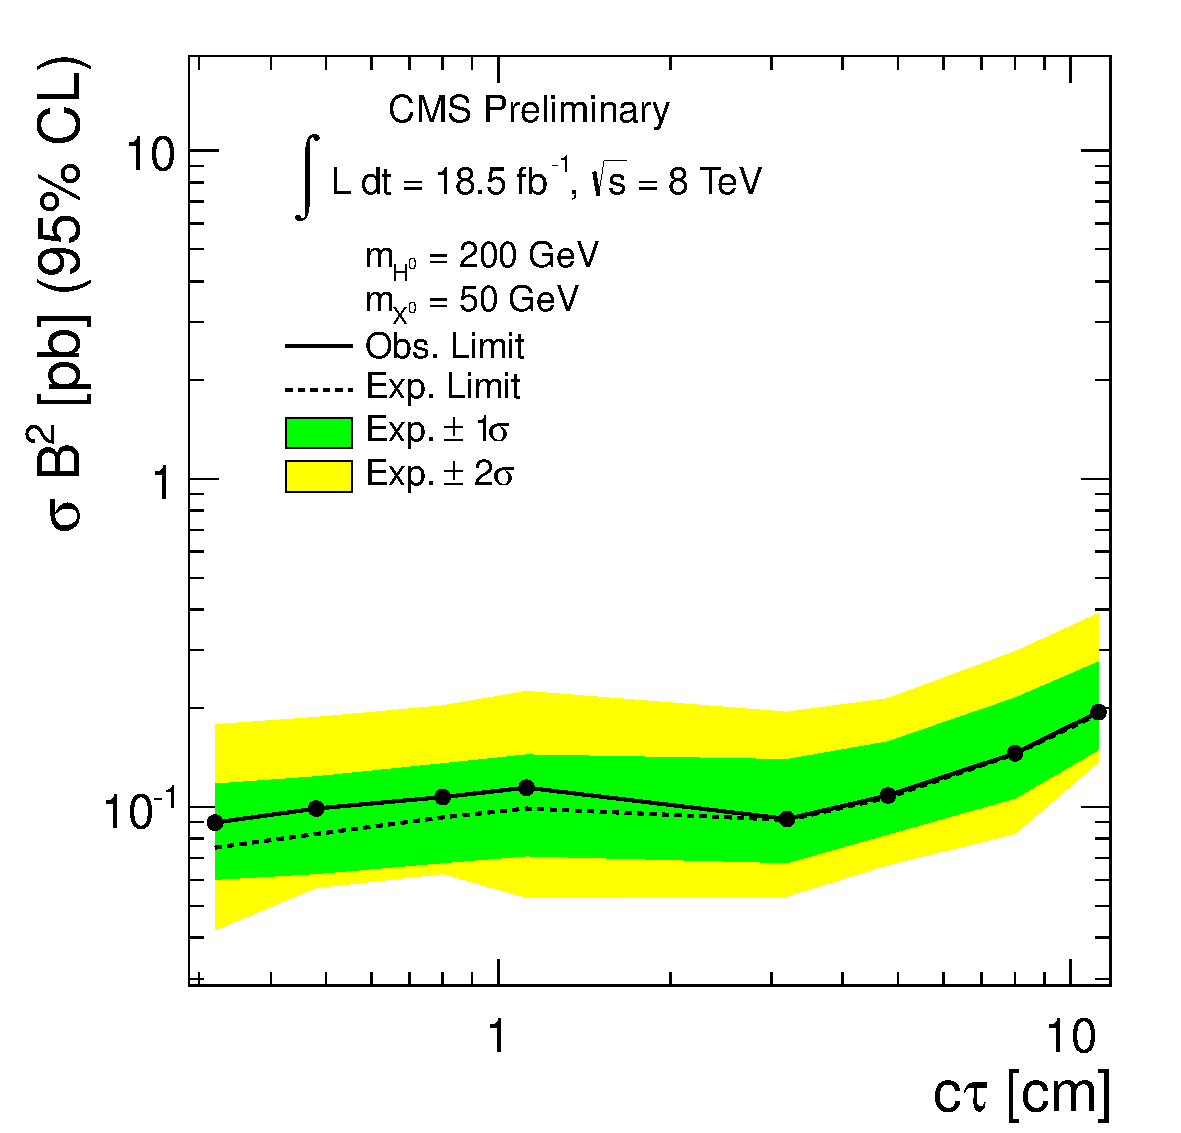
\includegraphics[width=0.49\textwidth]{plots/limits/200_50e.pdf}

\caption{Expected and observed 95\% CL limits for all tested signal models.\label{fig:limits}}
\end{figure}
